\chapter{Sistemas de arquivos}\label{cap:SistemasArquivos}

Arquivos são unidades lógicas de informação criadas por processos. Podemos pensar nos arquivos como espaços de endereçamento que são usados para modelar o disco em vez da memória \emph{RAM} os processos podem ler estes e através dos dados contidos neles gerar novos caso necessário. As informações contidas nos arquivos devem ser persistentes, ou seja, mesmo após o termino do processo elas devem ser mantidas integras para utilização futura exceto quando o próprio utilizador do sistema deseja excluir este. No \emph{Linux} os arquivos sofrem uma estrutura hierárquica onde podemos ter níveis de permissões variando entre proprietário, grupo ao qual o proprietário pertence e público (ou seja, qualquer usuário do sistema). Os arquivos normalmente possuem três operações básicas escrita, leitura e execução \cite{Morimoto2011}, \cite{guialinux2020}, \cite{luciano2015}.\\
Arquivos são gerenciados pelo sistema operacional. Como são estruturados, nomeados, acessados, usados, protegidos, implementados e gerenciados são tópicos importantes no projeto de um sistema operacional. Como um todo, aquela parte do sistema operacional lidando com arquivos é conhecida como sistema de arquivos.\\
Basicamente o sistema de arquivos é um conjunto de estruturas logicas que permite o sistema operacional controlar o acesso a um dispositivo de armazenamento, diferentes sistemas operacionais podem usam diferentes sistemas de arquivos, atualmente, o \emph{NTFS (New Technology File System)} é o sistema de arquivos padrão do \emph{Windows}, enquanto o \emph{ext4} é o do \emph{Linux} \cite{Morimoto2011}, \cite{guialinux2020}, \cite{luciano2015}.\\
\\Abaixo podemos ver alguns dos sistemas de arquivos mais conhecidos:\\
\\•	\emph{EXT3 (third extended filesystem)} – foi adotado como padrão \emph{Linux} a partir de 2001. Introduziu o registro \emph{(journal)} que melhora a confiabilidade e permite recuperar o sistema em caso de desligamento não programado. \emph{EXT3} suporta 16TB (1 terabyte corresponde a 240 bytes) de tamanho máximo no sistema de arquivos, e 2TB de tamanho máximo de um arquivo. Um diretório pode ter, no máximo, 32.000 subdiretórios.\\
\\•	\emph{EXT4 (fourth extended filesystem)} – passou a ser o padrão \emph{Linux} a partir de 2008. \emph{EXT4} suporta 1EB (1 exabyte corresponde a 260 bytes) de tamanho máximo de sistema de arquivos e 16TB de tamanho máximo de arquivos. É possível ter um número ilimitado de subdiretórios.\\
\\•	\emph{XFS (Extended Filesystem)} – usado como padrão por algumas distribuições \emph{Linux} desde 2014. \emph{XFS} é um sistema de arquivos desenvolvido em 64 bits, compatível com sistemas de 32 bits. Ele suporta até 16 EB de tamanho total do sistema de arquivos e até 8 EB de tamanho máximo para um arquivo individual. É considerado um sistema de arquivos de alto desempenho.\\
\\•	\emph{JFS (Journaled File System)} – é um sistema de arquivos de 64 bits com \emph{journaling} desenvolvido pela \emph{IBM}.\\
\\•	\emph{HFS (Hierarchical File System)} – é um sistema de arquivos proprietário da \emph{Apple}.\\
    \\•	\emph{FAT (File Allocation Table)} – é um sistema desenvolvido para o \emph{MS-DOS} e usado em versões do \emph{Microsoft Windows} até o \emph{Windows 95}. É suportado praticamente por todos os sistemas operacionais existentes. Existem 3 versões do sistema: \emph{FAT} (12 bits, usado pelos disquetes), \emph{FAT16} (para OS 16 bits ou 32 bits) e \emph{FAT32} (só para SO a 32 bits).\\
\\•	\emph{NTFS (New Technology File System)} é o sistema de arquivos padrão do sistema operacional \emph{Microsoft Windows}. São algumas características deste tipo de sistema: aceita volumes de até 2 TB; o tamanho do arquivo é limitado apenas pelo tamanho do volume; é um sistema de arquivos muito mais seguro que o \emph{FAT}; \emph{NTFS }podem se recuperar de um erro mais facilmente.\\
\\•	\emph{HPFS} –  é o sistema de arquivos utilizado pelo \emph{OS/2} da \emph{IBM}, com recursos que se aproximam muito dos permitidos pelo \emph{NTFS}.\\
\\•	\emph{UFS (Unix File System)} – é um sistema de arquivos usados por muitos sistemas operacionais \emph{Unix} e assemelhados \cite{Morimoto2011}, \cite{guialinux2020}, \cite{luciano2015}.\\

\section{Gerenciamento de diretório}

Sistemas de arquivos normalmente têm diretórios ou pastas, que podem ser de nível único ou hierárquicos.\\
Segundo Tanenbaum(2016) a forma mais simples de um sistema de diretório é ter um diretório contendo todos os arquivos. Às vezes ele é chamado de diretório-raiz. \\Essa decisão foi tomada sem dúvida para manter simples o \emph{design} do \emph{software}. Um exemplo de um sistema com um diretório é dado na Figura \ref{fig:DiretorioRaiz}. Aqui o diretório contém quatro arquivos. As vantagens desse esquema são a sua simplicidade e a capacidade de localizar arquivos rapidamente às vezes ele ainda é usado em dispositivos embarcados simples como câmeras digitais e alguns \emph{players} portáteis de música \cite{Tanenbaum2016}. \\\\

\begin{figure}[htpb]
    \centering
   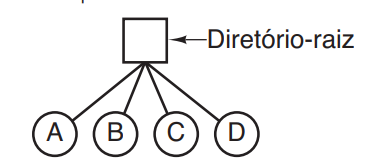
\includegraphics[scale=1]{imagens/DiretorioRaiz.png}
   \caption{Um sistema de diretório em nível único contendo
   quatro arquivos. \cite{Tanenbaum2016}}
   \label{fig:DiretorioRaiz}
\end{figure} 

Apesar do método anterior ser mais simples em atualmente os usuários em seus dispositivos milhares de arquivos inviabilizando o modelo anterior em consequência, é necessária uma maneira para agrupar arquivos relacionados em um mesmo local\cite{Tanenbaum2016}. 
Faz-se necessária uma hierarquia (isto é, uma árvore de diretórios). Com essa abordagem, o usuário pode ter tantos diretórios quantos forem necessários para agrupar seus arquivos de maneira natural. 
Além disso, se múltiplos usuários compartilham um servidor de arquivos comum, como é o caso em muitas redes de empresas, cada usuário pode ter um diretório-raiz privado para sua própria hierarquia. Essa abordagem é mostrada na Figura \ref{fig:DiretorioRaiz2} \cite{Tanenbaum2016}. 

\begin{figure}[htpb]
    \centering
   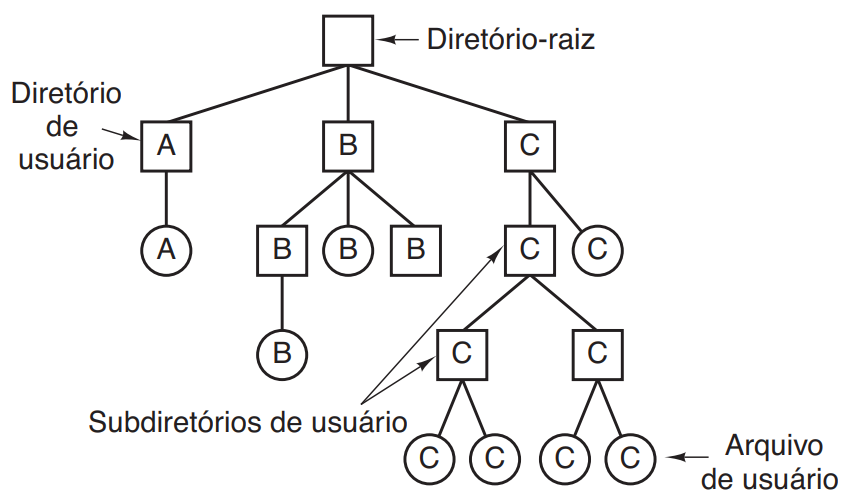
\includegraphics[scale=0.7]{imagens/DiretorioRaiz2.png}
   \caption{Um sistema hierárquico de diretórios. \cite{Tanenbaum2016}}
   \label{fig:DiretorioRaiz2}
\end{figure} 

No \emph{Linux} o diretório raiz e o diretório “/” é o diretório com maior hierarquia entre todos os diretórios do sistema assim todos os outros diretórios estão abaixo dele\cite{Morimoto2011}, \cite{guialinux2020}, \cite{luciano2015}.\\ \\
\\A seguir são apresentados exemplos de diretórios que normalmente ficam abaixo do diretório raiz.\\
•	bin – diretório com os comandos disponíveis para os usuários comuns (não privilegiados).\\
•	boot – diretório com os arquivos estáticos do \emph{boot} de inicialização.\\
•	dev – diretório com as definições dos dispositivos de entrada/saída.\\
•	etc – diretório com os arquivos de configuração do sistema.\\
•	home – diretório que armazena os diretórios dos usuários do sistema.\\
•	lib – diretório com as bibliotecas e módulos (carregáveis) do sistema.\\
•	lost+found – é usado pelo \emph{fsck} para armazenar arquivos/diretórios/devices corrompidos.\\
•	media – ponto de montagem temporário para mídias removíveis.\\
•	mnt – ponto de montagem temporário para sistemas de arquivos.\\
•	opt – \emph{softwares} adicionados pelos usuários.\\
•	proc – diretório com informações sobre os processos do sistema.\\
•	root – diretório \emph{home do root}.\\
•	run – armazena arquivos temporários da inicialização do sistema.\\
•	sbin – diretório com os aplicativos usados na administração do sistema.\\
•	snap – diretório com pacotes snaps (podem ser executados em diferentes distribuições \emph{Linux}).\\
•	srv – dados para serviços providos pelo sistema.\\
•	sys – contém informações sobre \emph{devices, drivers} e características do \emph{kernel}.\\
•	tmp – diretório com arquivos temporários.\\
•	usr – diretório com aplicativos e arquivos utilizados pelos usuários como, por exemplo, o sistema de janelas X, jogos, bibliotecas compartilhadas, programas de usuários e de administração, etc.\\
•	var – diretório com arquivos de dados variáveis (\emph{spool, logs}, etc).\\
\\Três comandos básicos do \emph{Linux server} para se deslocar entre diretórios são:\\
\\\emph{pwd (print working directory)}: informa o diretório de trabalho - ou corrente, apresentando o caminho desde o raiz até o diretório atual.\\
\\\emph{ls (list space)}: lista, de maneira simples ou com informações variadas, arquivos específicos ou o conteúdo de diretórios.\\
\\\emph{cd (change directory)}: serve para fazer a mudança entre os diretórios - como o próprio nome informa o seu uso pode ser para caminhar na pasta local, dentro da própria pasta, ou para qualquer local do sistema.\\
\\Compartilhamento de arquivos muitas vezes é necessário que um arquivo se mostre simultaneamente em diretórios diferentes por estar compartilhado entre vários usuários ou por possuir informação que são necessárias para o sistema como na figura \ref{fig:DiretorioRaiz3} abaixo \cite{Tanenbaum2016}: 

\begin{figure}[htpb]
    \centering
   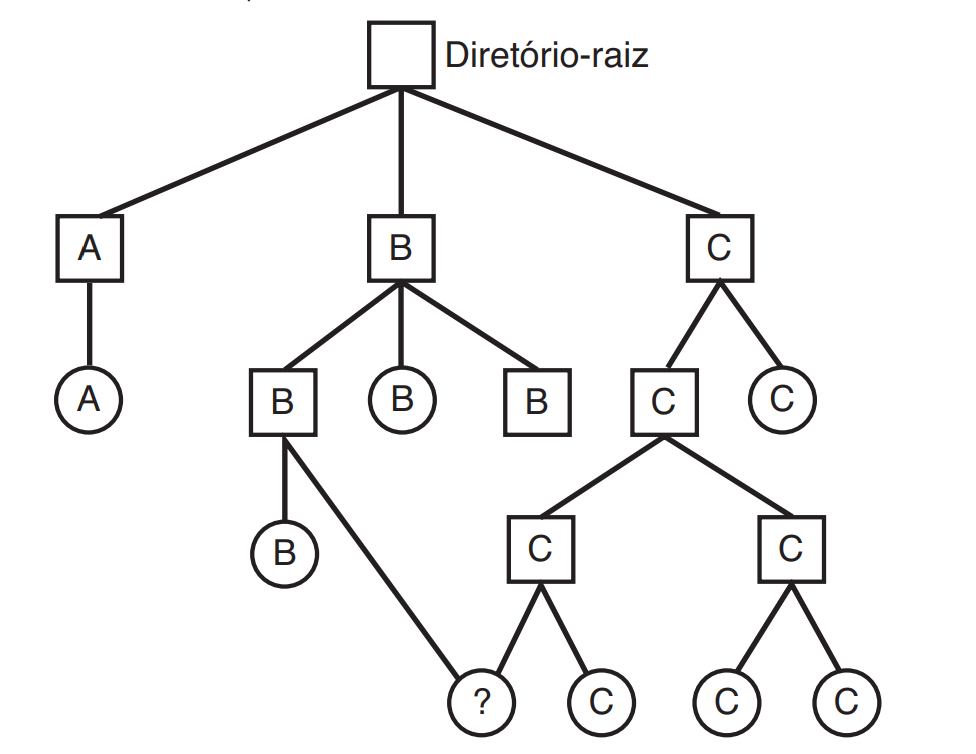
\includegraphics[scale=0.55]{imagens/DiretorioRaiz3.png}
   \caption{Sistema de arquivos contendo um arquivo
   compartilhado.  \cite{Tanenbaum2016}}
   \label{fig:DiretorioRaiz3}
\end{figure} 

O compartilhamento de arquivos pode gerar alguns problemas se os diretórios realmente contiverem endereços de disco, então uma cópia desses endereços terá de ser feita no diretório do de cada usuário quando o arquivo for utilizado subsequentemente se cada usuário adicionarem blocos de arquivos em seu diretório pessoal quando utilizarem o arquivo é praticamente como se o usuário estivesse copiando o arquivo para seu diretório assim perdendo o sentido do compartilhamento \cite{Tanenbaum2016}.\\
Segundo Tanenbaum(2016) ele diz que esse problema pode ser solucionado de duas maneiras. Na primeira solução, os blocos de disco não são listados em diretórios, mas em uma pequena estrutura de dados associada com o arquivo em si. Os diretórios apontariam então apenas para a pequena estrutura de dados. Essa é a abordagem usada em \emph{UNIX} (em que a pequena estrutura de dados é o \emph{i-node}).
A segunda solução seria que quando um novo usuário utilize do arquivo seja criado um arquivo \emph{link} que irá conter apenas uma receita do arquivo original contendo seu o caminho do arquivo que está sendo utilizado, essa abordagem é chamada de ligação simbólica \cite{Tanenbaum2016}.

\section{Gestão de espaço livre}

Arquivos são armazenados em disco e os discos possuem limites físicos quanto a tamanho do disco e quantidade de arquivos que podem ser armazenados. Visto isso o gerenciamento do espaço do disco é uma das preocupações do projetista de sistemas de arquivos \cite{Tanenbaum2016}. \\
O primeiro consiste em usar uma lista encadeada de blocos de disco, com cada bloco contendo tantos números de blocos livres de disco quantos couberem nele. Com um bloco de 1 KB e um número de bloco de disco de 32 bits, cada bloco na lista livre contém os números de 255 blocos livres \cite{Tanenbaum2016}.\\
A outra técnica de gerenciamento de espaço livre é o mapa de bits. Um disco com n blocos exige um mapa de bits com n bits. Blocos livres são representados por 1s no mapa, blocos alocados por 0s (ou vice-versa) \cite{Tanenbaum2016}.\\ Para nosso disco de 1 TB de exemplo, precisamos de 1 bilhão de bits para o mapa, o que exige em torno de 130.000 blocos de 1 KB para armazenar \cite{Tanenbaum2016}.\\ Não surpreende que o mapa de bits exija menos espaço, tendo em vista que ele usa 1 bit por bloco, versus 32 bits no modelo de lista encadeada.  

\begin{figure}[htpb]
    \centering
   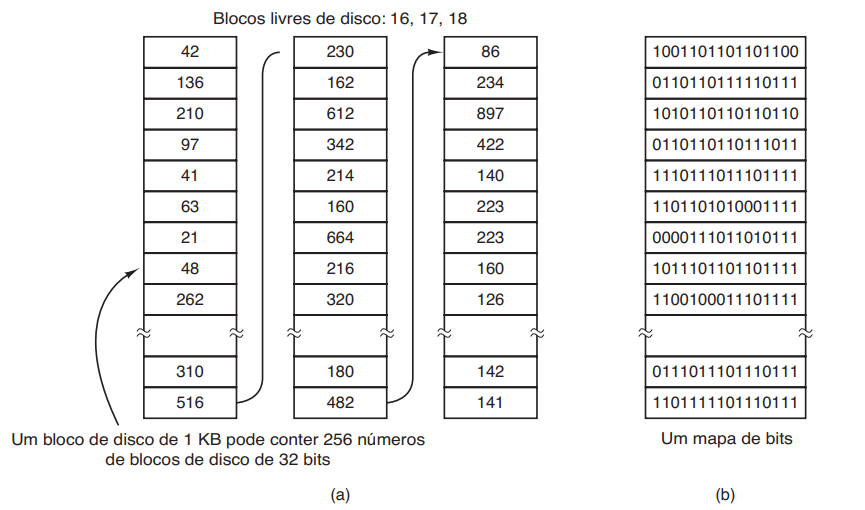
\includegraphics[scale=.8]{imagens/GestaoLivre.png}
   \caption{(a) Armazenamento da lista de blocos livres em uma lista encadeada. (b) Um mapa de bits. \cite{Tanenbaum2016}}
   \label{fig:GestaoLivre}
\end{figure} 

\section{Cotas de disco}

É comum em sistemas de multiusuários que os sistemas definam cotas de disco que é um mecanismo para impor um tamanho máximo de utilização para cada usuário assim ele impede que o usuário utilize o sistema de forma a prejudicar o funcionamento do sistema\cite{Tanenbaum2016}. \\. 
Quando um usuário abre um arquivo é gerada uma tabela de arquivos aberta na memória principal com os atributos endereços de disco são localizados. Quaisquer aumentos no tamanho do arquivo serão cobrados da cota do proprietário, uma segunda tabela é contendo os registros de cotas de todos os usuários com um arquivo aberto, mesmo que esse arquivo tenha sido aberto por outra pessoa. Essa tabela está mostrada na Figura \ref{fig:CotaDisco}. Ela foi extraída de um arquivo de cotas no disco para os usuários cujos arquivos estão atualmente abertos. Quando todos os arquivos são fechados, o registro é escrito de volta para o arquivo de cotas. Quando uma nova entrada é feita na tabela de arquivos abertos, um ponteiro para o registro de cota do proprietário é atribuído a ela, a fim de facilitar encontrar os vários limites \cite{Tanenbaum2016}. \\
Toda vez que um bloco é adicionado a um arquivo, o número total de blocos cobrados do proprietário é incrementado, e os limites flexíveis e estritos são verificados. O limite flexível pode ser excedido, mas o limite estrito não. Esse método tem a propriedade de que os usuários podem ir além de seus limites flexíveis durante uma sessão de uso, desde que removam o excesso antes de se desconectarem. Os limites estritos jamais podem ser excedidos \cite{Tanenbaum2016}.

\begin{figure}[htpb]
    \centering
   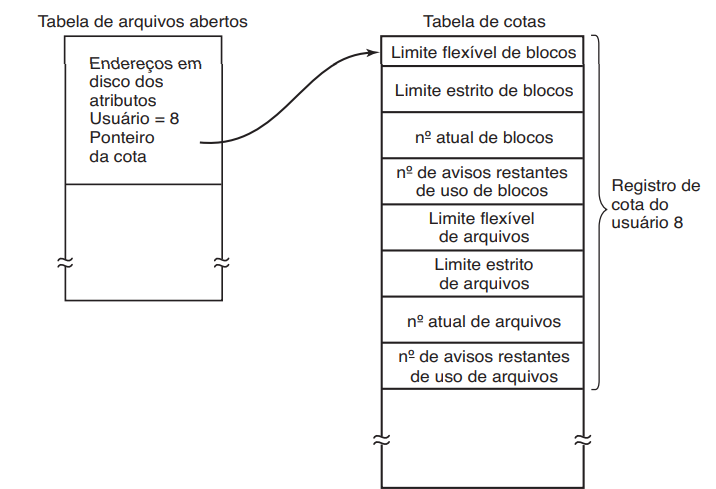
\includegraphics[scale=0.6]{imagens/CotaDisco.png}
   \caption{As cotas são relacionadas aos usuários e monitoradas em uma tabela de cotas. \cite{Tanenbaum2016}}
   \label{fig:CotaDisco}
\end{figure} 